
\documentclass[11pt,a4paper]{scrartcl}
\usepackage[utf8]{inputenc}
\usepackage[english]{babel}
\usepackage{microtype}
\usepackage{amsmath}
\usepackage{mathtools}
%\usepackage[leqno]{amsmath}
\usepackage{amsfonts}
\usepackage{amssymb}
\usepackage{graphicx}
\usepackage{indentfirst}
\usepackage{fancyvrb}
%\usepackage{subfigure}
\usepackage{caption}
\usepackage{subcaption}
\usepackage{enumitem}
\usepackage{booktabs}
\usepackage{algorithm}
\usepackage{algpseudocode}
\usepackage[onehalfspacing]{setspace}
\usepackage[hidelinks]{hyperref}
\usepackage{listings}
\usepackage{xcolor}
\usepackage{fancyhdr}
\pagestyle{fancy}
\fancyhf{}
\fancyhead[R]{\thepage}

\usepackage{amsmath}
\usepackage{nccmath}
\newenvironment{mpmatrix}{\begin{medsize}\begin{pmatrix}}%
{\end{pmatrix}\end{medsize}}%

\date{}
\title{STDP-based spiking deep convolutional neural networks for object recognition}
\begin{document}

\begin{titlepage}
\begin{center}
	
\includegraphics[scale=0.8]{images/SapienzaLogo} \\
	\vspace{3em}
	{\large \textsc{Facoltà di  Ingegneria dell'informazione, Informatica e Statistica}} \\
	\vspace{2em}
	{\large \textsc{Neural Networks}} \\
	\doublespacing
	\vspace{5em}
	{\Large \textbf{STDP-based spiking deep convolutional neural networks for object recognition}}
\end{center}

\vskip 2cm
\begin{center}
\begin{tabular}{c c c c c c c c}
	Supervisor & & & & & & & Students \\[0.2cm]
	\large{Simone Scardapane} & & & & & & & \large{Edoardo Ghini}\\[0.2cm]
	\large{} & & & & & & & \large{Gianluca Cerilli}\\
	\end{tabular}
\end{center}

\vskip 1.5cm
\begin{center}
	{\normalsize Academic Year 2017/2018}
\end{center}
\end{titlepage}

\clearpage{\pagestyle{empty}\cleardoublepage}

\vspace{5em}

\onehalfspacing

\clearpage{\pagestyle{empty}\cleardoublepage}


\tableofcontents

\clearpage
\section*{Introduction}
Second generation artificial neural networks -- mainly characterized by fully connected layers that deal with continuous output values -- have allowed us to make enormous progresses in many relevant scientific fields. In the same way, also the third generation of artificial neural networks seems to be very promising and it is expected to bridge the gap between neuroscience and machine learning by using more realistic \textit{spiking} neuron models. These third generation networks are called \textquotedblleft Spiking Neural Networks\textquotedblright and are different from usual networks, since they do not deal with continuous values, but they communicate through spikes, that are discrete events that occur at certain points in time.Indeed, when a (membrane of a) neuron reaches a certain potential value, it spikes, so it resets its value.
This behaviour is inspired by real biological processes and is expected to better model reality. This may seem not so \textquotedblleft innovative\textquotedblright, since discrete signals are used instead of continuous ones. Instead, this modelling allows us to handle spatio-temporal data, that are real-world sensory data. These spatial and temporal aspects refer to the fact that neurons are connected to neurons local to them and that temporal information of the spikes (that are lost in binary encoding) are now preserved. Indeed, it has been proven that spiking neurons are computationally more powerful than traditional artificial neurons.\\
In this report we describe a project in the frame of the \textquotedblleft Neural Networks\textquotedblright course of Sapienza Università di Roma, that is inspired from the \textquotedblleft STDP-based spiking deep convolutional neural networks for object
recognition\textquotedblright paper of Kheradpisheh, Ganjtabesh, Thorpe and Masquelier. In particular, the implementation of a Spiking Convolutional Neural Network for object classification is described.

\section{Network architecture}

An STDP-based spiking deep neural network (SDNN) with a spike-time neural coding has been implemented. In the very beginning of this network, the input image is passed to the temporal-coding layer,that uses Difference of Gaussians (DoG) filters to convert the image into an asynchronous spike train. This is used as input for the successive layer, that is a convolutional one,
in which input spikes are integrated and new spikes are emitted if a certain threshold is exceeded, that is when a visual feature is detected. Learning is done through STDP that is used to learn visual features, and so the weights of the network. Neurons that fire earlier in this phase prevent the others from firing. The convolutional layer is followed by a pooling one, where the visual information is compressed. Three convolutional and pooling layers (arranged in an alternate and consecutive order) have been implemented to handle larger and more complex visual features through the network. In the end, in the last pooling layer, a global max pooling is performed for the classification, to train a linear classifier. The results are used to find the proper category to which the input image belongs.\\
\begin{figure}[h]
	\centering
	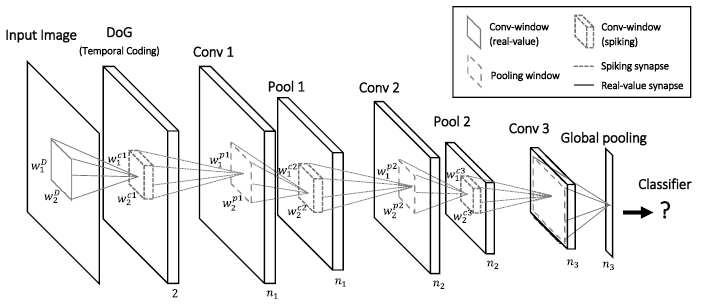
\includegraphics[width=\textwidth]{images/architecture}
	\caption{SDNN architecture}
	\label{fig:architecture}
\end{figure}

\subsection{Temporal coding}

In the very first part of the neural network, the input signal is encoded into temporal-discrete spike events. A Difference of Gaussians (DoG) filter is used to detect the contrasts in the input image and emit a spike, accordingly. The higher the contrast in a certain cell, the more strongly this one is activated in order to fire. The firing time (i.e. the time when the spike is emitted) of a DoG cell is inversely proportional to its activation value. In particular, if an \textit{r} output is obtained in a cell after DoG, its corresponding firing time will be $ \tau = 1/r $. DoG cells are sensitive to both positive and negative contrasts, depending on their two ON-centre and OFF-centre maps and they fire when their activation values exceed a predefined threshold.

\subsection{Convolutional and pooling layers}

A convolutional layer is represented by several neuronal maps, whose role is to detect visual features at different locations. To this extent, the synaptic weights assigned to the same neuronal map will be the same. Each neuron in the convolutional layer generates spikes according to what it receives from the pre-synaptic neurons and when its internal membrane potential reaches a certain threshold. So, at each time step \textit{t}:
\begin{equation*}
	V_{i}(t) = V_{i}(t-1) + \sum_{j}W_{j,i}S_{j}(t-1)
\end{equation*}
the internal potential $ V_{i}(t) $ of the \textit{i-th} convolutional neuron is updated by adding the spike train $ S_{j}(t-1) $ of the \textit{j-th} pre-synaptic neuron, multiplied by the synaptic weight $ W_{j,i} $ between the \textit{j-th} pre-synaptic neuron and \textit{i-th} convolutional neuron. In particular, $ S_{j}(t-1) $ can be equal to 1 if the neuron has fired at previous time, or to 0 otherwise. If the neuron potential $ V_{i}(t) $ exceeds the threshold $ V_{th} $, then the neuron emits a spike ($ S_{i}(t) = 1 $) and resets its potential to zero. After it fires, the neuron can not fire again and it also inhibits other neurons in its same location (but belonging to other neuronal maps). In this way it is easier to detect a visual feature in a certain location.\\
In the pooling layer instead, each neuron performs a max pooling operation over a window in the corresponding neuronal map of the previous layer. Here no learning occurs and, as before, each neuron can emit only one spike. In this phase the visual information is compressed. These convolution and pooling phases are repeated for three times, to handle larger and always more complex data.

\subsection{STDP-based learning}

Spike-timing-dependent plasticity (STDP) is actually a biological process used by brain to modify its own synapses. This same idea has been also used in neural networks, so as to have stronger synapses in case they contribute to the firing of a post-synaptic neuron and weaker synapses if they do not give any contribute to the firing.\\
\begin{figure}[h]
	\centering
	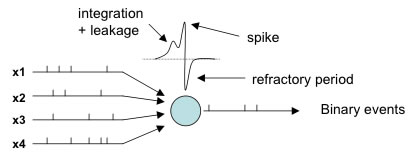
\includegraphics[width=0.75\linewidth]{images/spikes}
	\caption{Contributon to the firing of a post-synaptic neuron}
	\label{fig:spikes}
\end{figure}\\
This process is easy to understand by looking at figure \ref{fig:spikes}. In this case, four different pre-synaptic neurons are connected to one neuron (the blue one) by synapses. Each of them is characterized by its own firing rate. These spikes are sent forward by the corresponding synapses so as to increase the membrane potential of the post-synaptic neuron. When the latter spikes, it is possible to see which pre-synaptic neuron has contributed and its membrane potential is increased. In the same way, the potentials of the neurons that have not contributed to the firing of the post-synaptic one, are weakened.\\
As already mentioned, learning occurs only in convolutional layers, so that neurons compete to fire earlier than others and use STDP to learn input patterns. This competition is crucial to encourage neurons of different neuronal maps to learn different features. In this case, STDP is represented by:
\begin{equation*}
	\Delta w_{ij} = \begin{cases}
		a^{+}w_{ij}(1-w_{ij}), & \textit{if }\; t_{j}-t_{i} \leq 0,\\
		a^{-}w_{ij}(1-w_{ij}), & \textit{if }\; t_{j}-t_{i} > 0,
	\end{cases}
\end{equation*}
where \textit{i} and \textit{j} refer to the pre-synaptic and post-synaptic neurons, respectively, $ \Delta w_{ij} $ is the synaptic weight modification and $ a^{+} $ and $ a^{-} $ are the learning rate parameters. The term $ w_{ij}(1-w_{ij}) $ is needed to bound the weight values between 0 and 1. The best choice for the learning rate parameters is with $ a^{+} $ greater than $ a^{-} $, with small values for both. This, to prevent that neurons learn more than one pattern and to allow them to reach the predefined threshold to fire.\\
It could happen that different neurons fire at the same time, because of the discrete time. In that case, the neuron with the highest potential is selected, since it should define a higher similarity between its learned feature and input pattern.\\
Weights are randomly initiated with mean 0.8 and standard deviation 0.05 and the learning convergence of the \textit{l-th} convolutional layer is represented by:
\begin{equation*}
C_{l} = \sum_{f}\sum_{i}w_{f,i}(1-w_{f,i})/n_{w}
\end{equation*}
where $ n_{w} $ is the total number of synaptic weights in that layer and $ w_{f,i} $ is the \textit{i-th} synaptic weight of the \textit{f-th} feature.

\subsection{Classification}
The output of the global max pooling layer is used to build a dataset of labelled features which are split in a training and testing set for the classifier. These features are characterized by a vector of 20 elements that represent the greatest potentials reached by the neuronal maps in the third convolutional layer. Indeed, the activation threshold of the neurons belonging to the last layer has been set to an infinite positive value, since it has been chosen to not incur the reset of the potentials, due to neurons spiking.\\
The resulting dataset is then standardised and used to feed a linear SVM.

\section{Results}

The spiking convolutional network has been evaluated on two main image categories: human faces and motorbikes. This dataset of 470 images has been divided into three main sets for the learning, training and testing phases, respectively.\\
At the beginning of the network, the input image (face or motor) is passed to the DoG filter that encodes the temporal information in 10 different layers. In the two images at the top of figure \ref{fig:face}, it is possible to see the input image and the contrasts highlighted by the DoG. The remaining four images instead, represent the first four outputs of the filter in which the information is encoded into discrete spike events. It is evident that the information is accumulated by augmenting the encoding layers.
\begin{figure}[!h]
	\centering
	\begin{minipage}[b]{0.685\textwidth}
		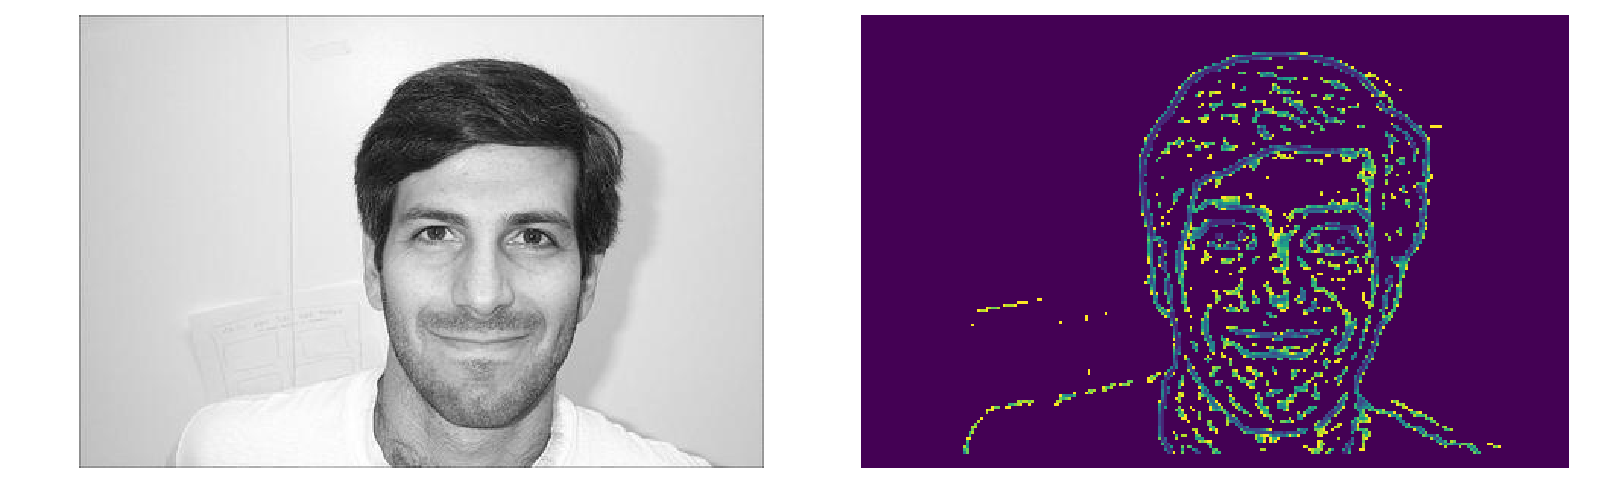
\includegraphics[width=\textwidth]{images/face_temp}
	\end{minipage}
	\\
	\begin{minipage}[b]{0.685\textwidth}
		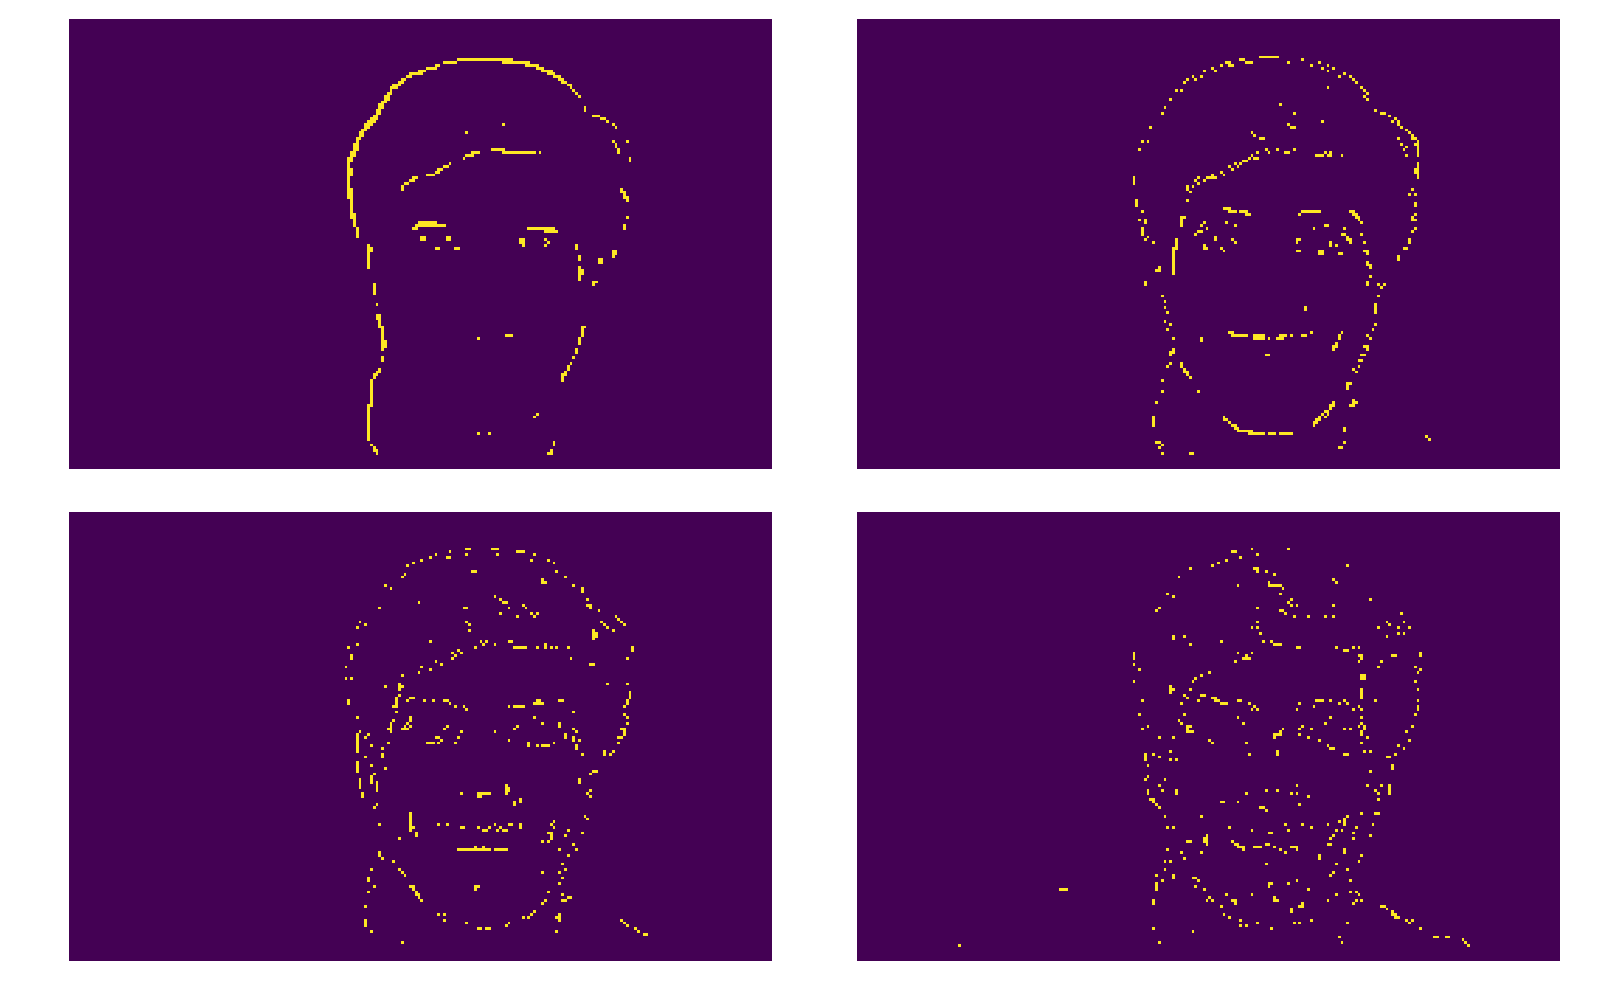
\includegraphics[width=\textwidth]{images/face_dog_out}
	\end{minipage}
	\caption{DoG temporal coding (face). Top-left: input image. Top-right: contrasts. Four images: first four encoding layers.}
	\label{fig:face}
\end{figure}\\
In the same way, it is possible to see the DoG outputs for the \ref{fig:motor} category.\\
\begin{figure}[!h]
	\centering
	\begin{minipage}[b]{0.685\textwidth}
		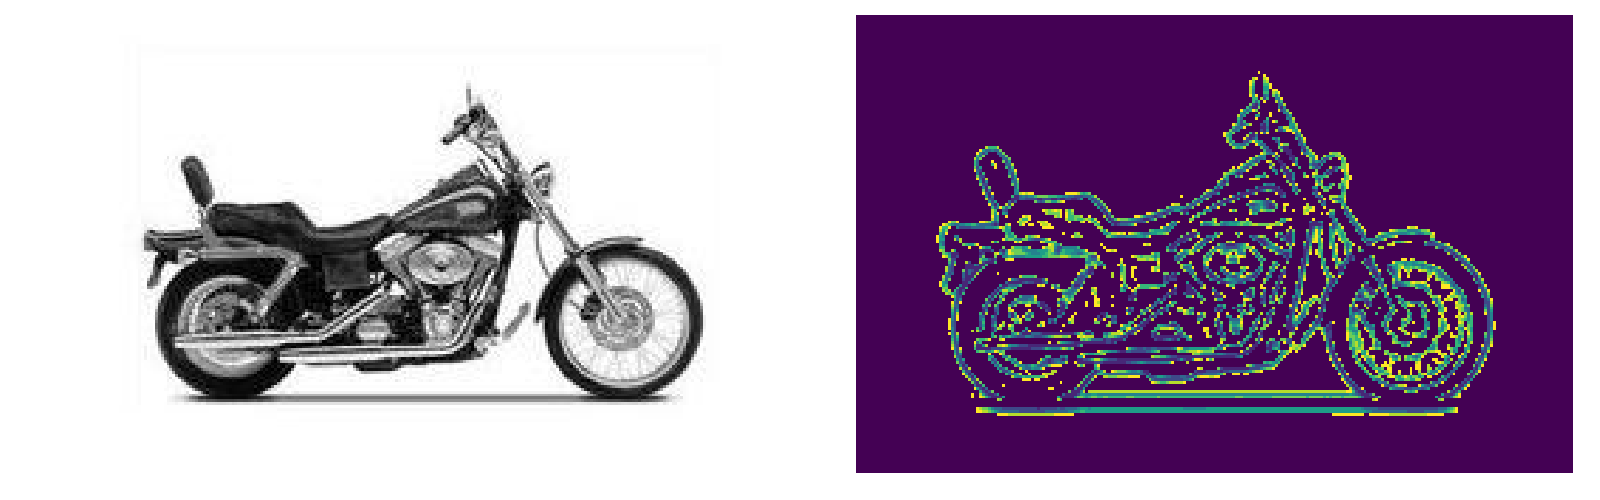
\includegraphics[width=\textwidth]{images/motor_temp}
	\end{minipage}
	\\
	\begin{minipage}[b]{0.685\textwidth}
		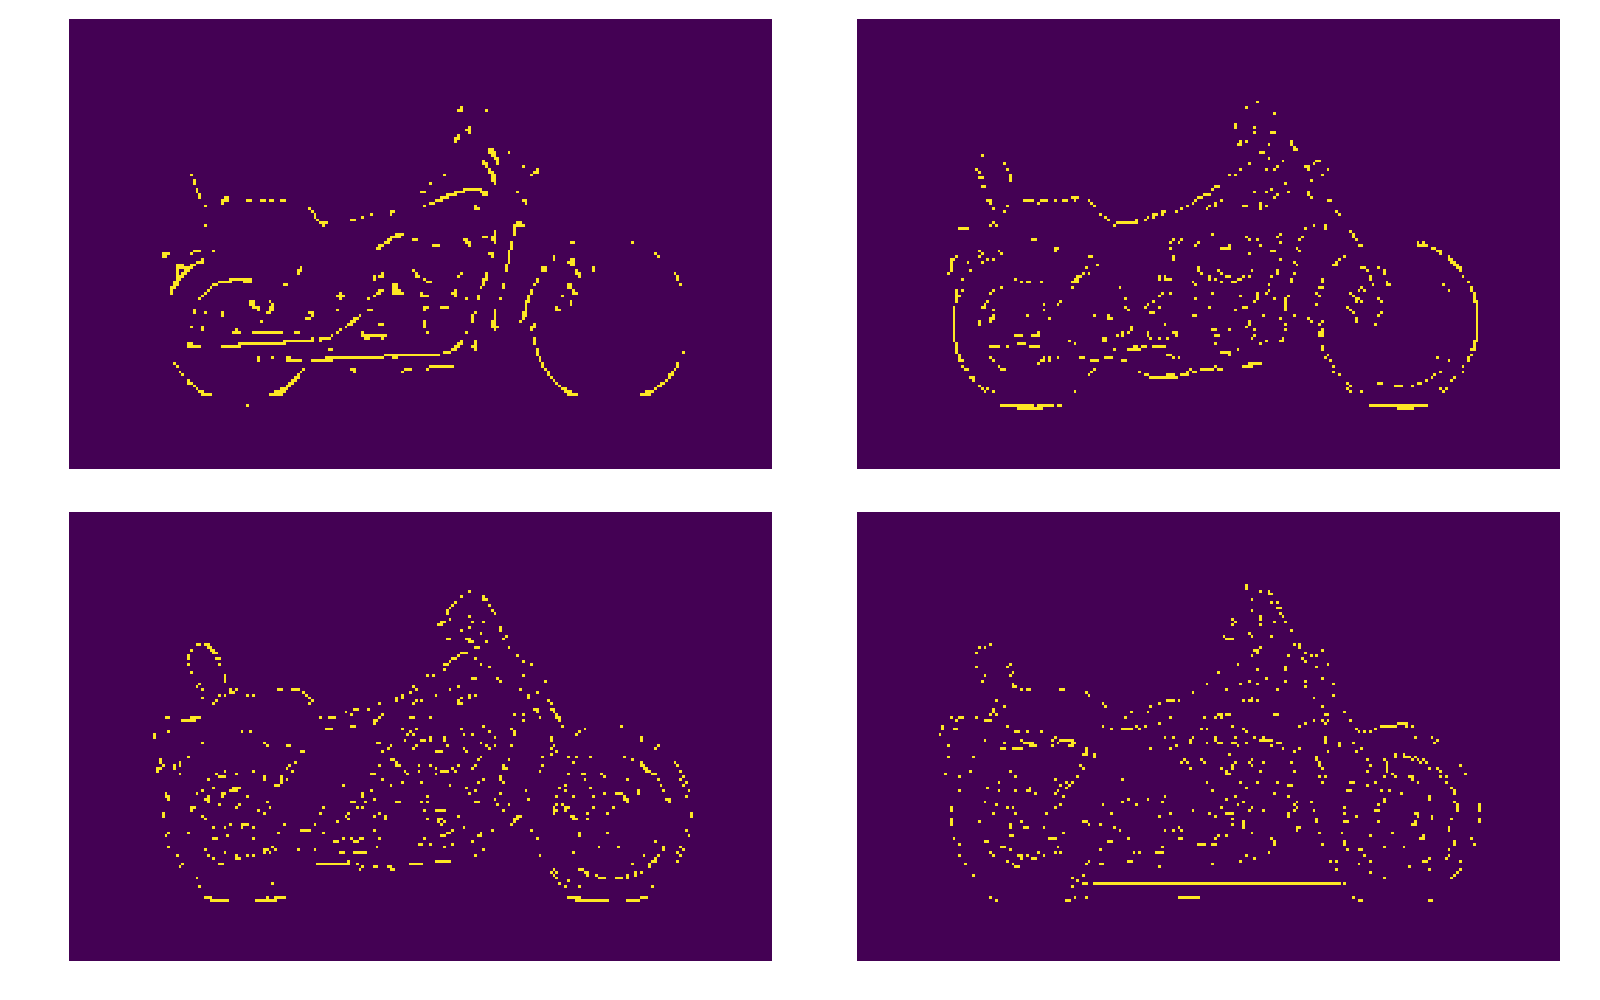
\includegraphics[width=\textwidth]{images/motor_dog_out}
	\end{minipage}
	\caption{DoG temporal coding (motorbike). Top-left: input image. Top-right: contrasts. Four images: first four encoding layers.}
	\label{fig:motor}
\end{figure}\\
By iterating over the DoG output images, these are passed in sequence to the convolutional layer. The latter is defined by a $ 16\times250\times1 $ input dimension, $ 5\times5 $ filter,  input and output channel equal to 1 and 4, respectively.
Four different output images are produced, that is possible to observe in figure \ref{fig:conv_out}. 
\begin{figure}[!h]
	\centering
	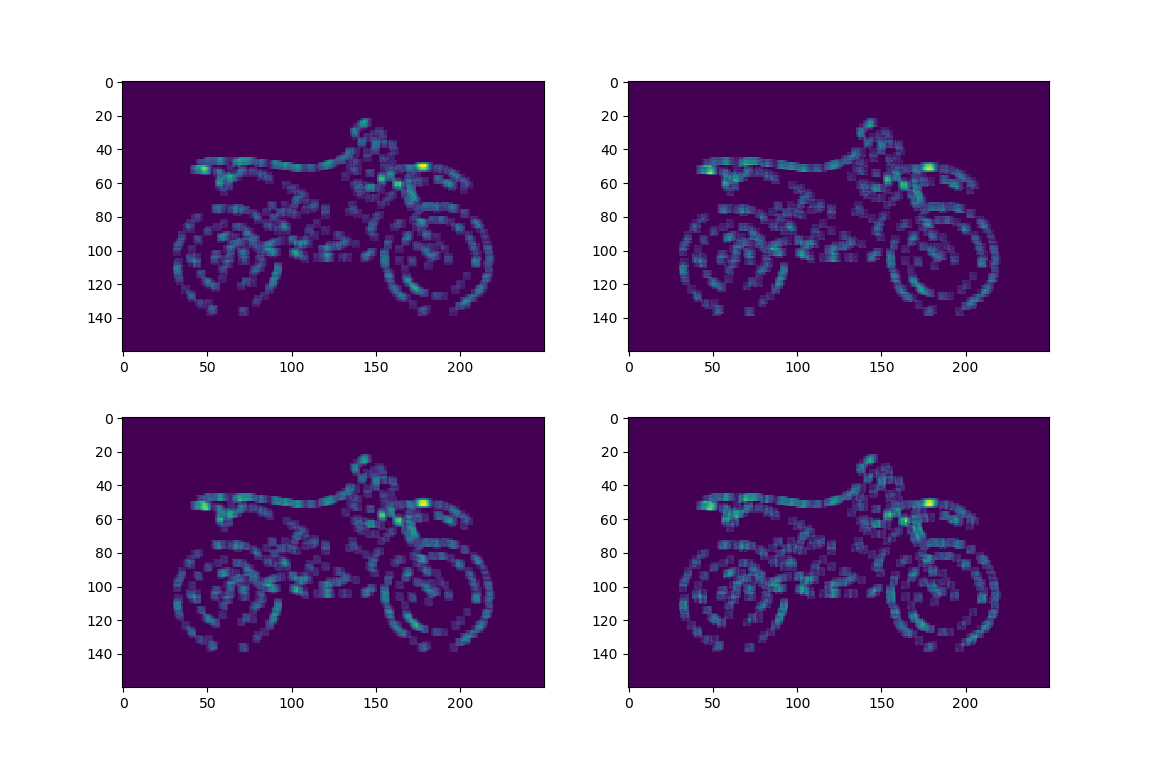
\includegraphics[width=\textwidth]{images/conv_output_slice3_cut}
	\caption{Output of the first convolutional layer}
	\label{fig:conv_out}
\end{figure}\\
It can be interesting to see what are the neurons that spike right after the convolution. This information is reported in figure \ref{fig:s_k}, in which it is possible to see the spiking neurons before inhibition -- the yellow pixels in the first four images at the top -- and after the inhibition -- the yellow pixels in the first four images at the bottom. The latter are less than the former, since the inhibition process resets the redundant spikes. The two yellow images to the right instead, represent the future spikes that will be reset, since the information has been already acquired.\\
\begin{figure}[!h]
	\centering
	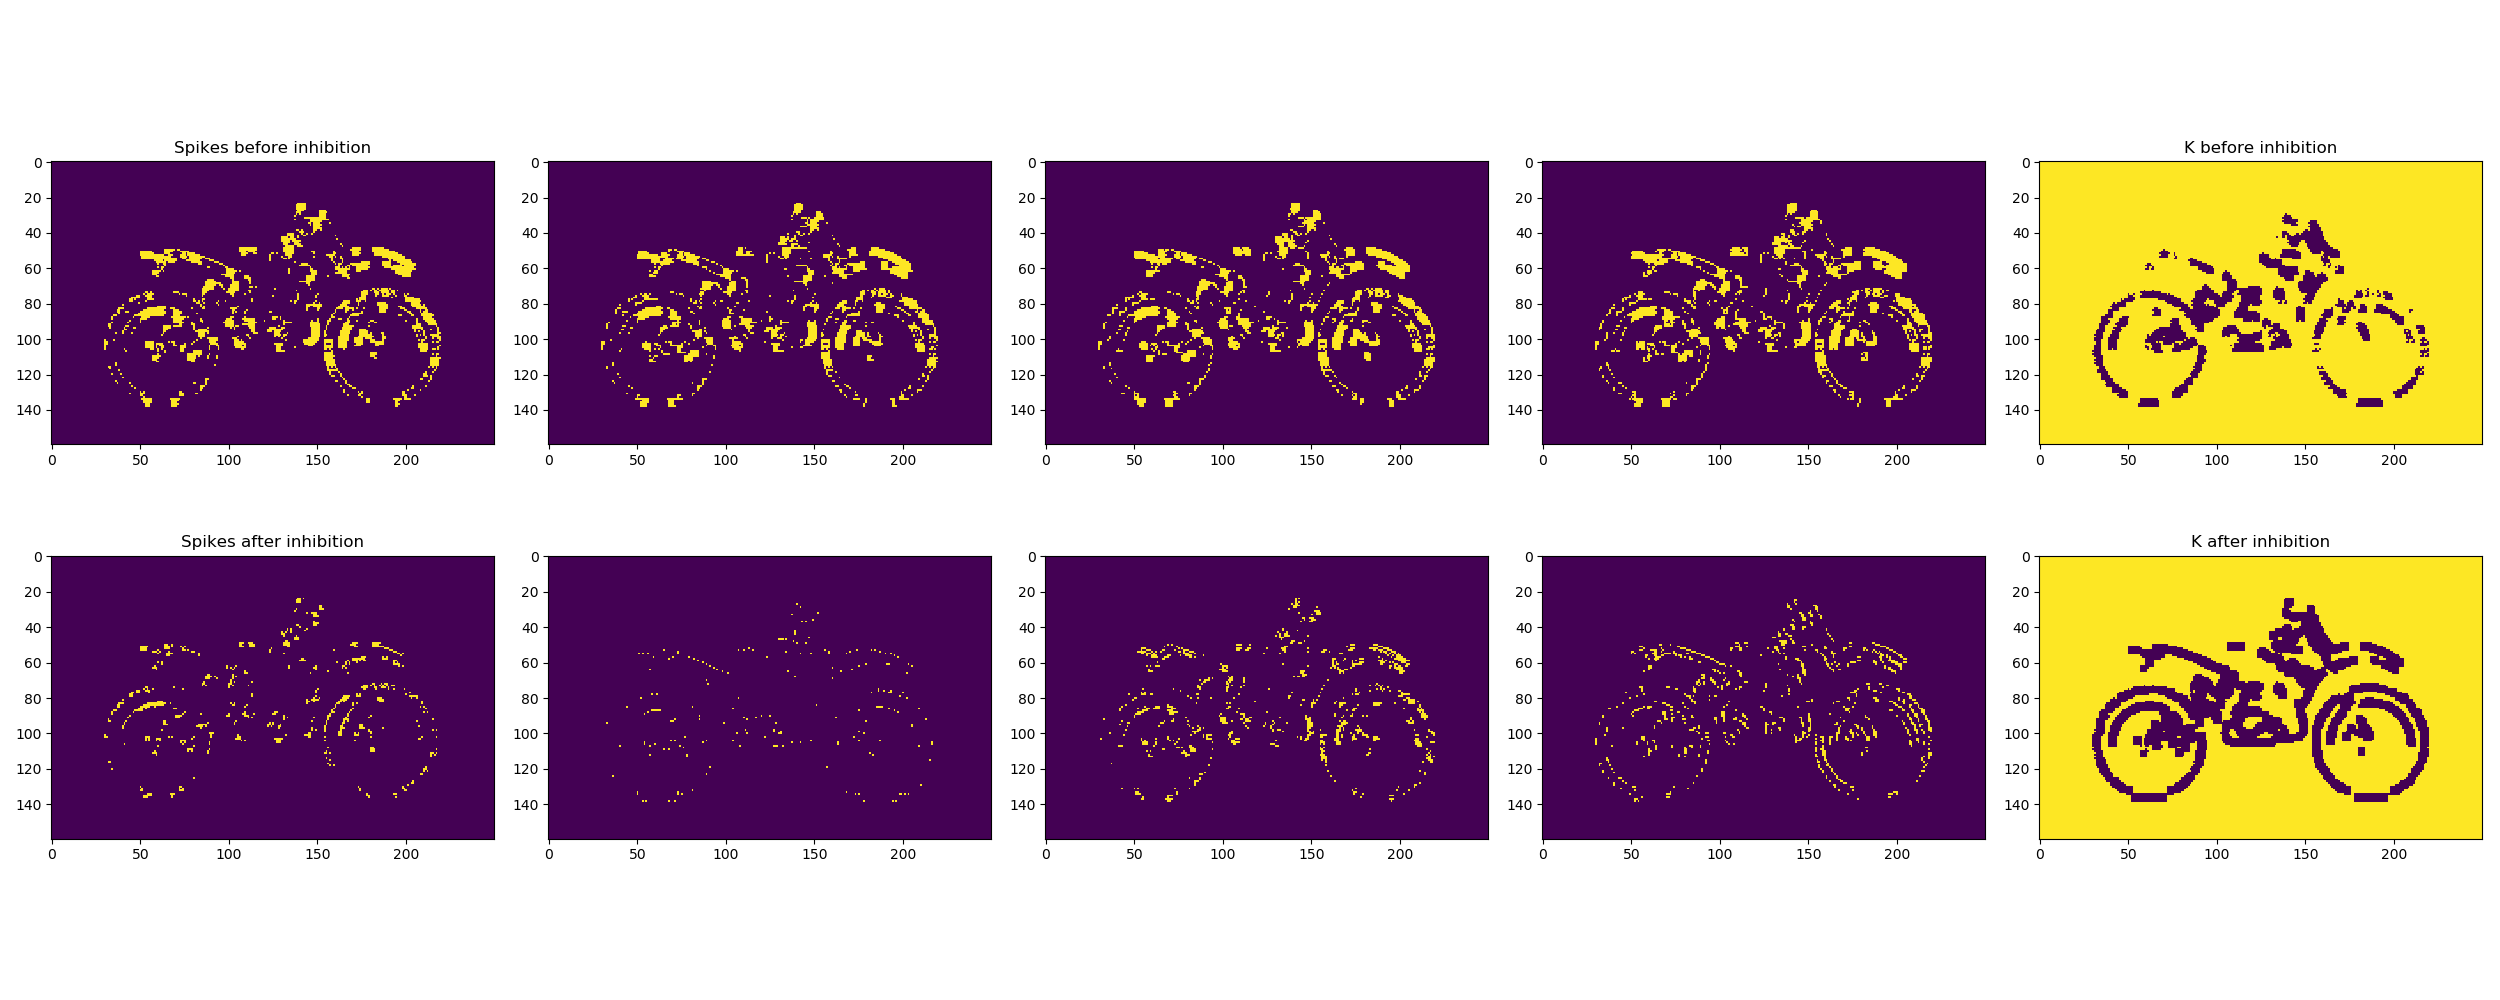
\includegraphics[width=\textwidth]{images/S_K_values_slice2}
	\caption{Top-left (four images): spiking neurons before inhibition. Bottom-left (four images): spiking neurons after inhibition. Right (yellow background images): location of the spikes that will be inhibited in the next step.}
	\label{fig:s_k}
\end{figure}\\
\newpage
By observing figure \ref{fig:k} it is possible to understand which neurons have been considered up to the current time, for the first three outputs of the DoG filter.\\
\begin{figure}[!h]
	\centering
	\begin{minipage}[b]{0.32\textwidth}
		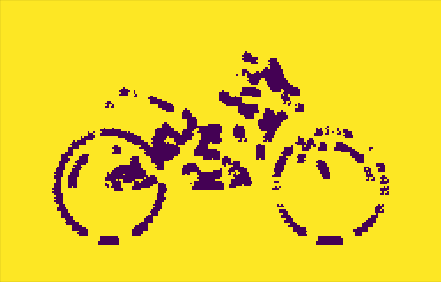
\includegraphics[width=\textwidth]{images/K_1}
	\end{minipage}
	\hfill
	\begin{minipage}[b]{0.32\textwidth}
		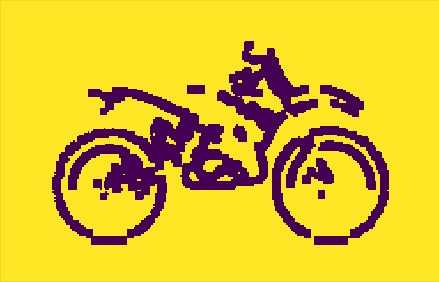
\includegraphics[width=\textwidth]{images/K_2}
	\end{minipage}
	\hfill
	\begin{minipage}[b]{0.32\textwidth}
		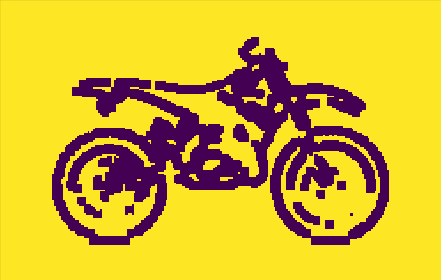
\includegraphics[width=\textwidth]{images/K_3}
	\end{minipage}
	\caption{Inhibition matrix for the first three outputs of the DoG filter}
	\label{fig:k}
\end{figure}\\
The four outputs of the convolutional layer are then passed to the pooling payer. This is defined by a $ 16\times250\times4 $ input dimension, a $ 7\times7 $ window shape and stride equal to $ 6 $. This operates a max pooling operation and produces the output shown in figure \ref{fig:pool}. It is easy to see how the visual information is compressed in the four images at the bottom.
\begin{figure}[!h]
	\centering
	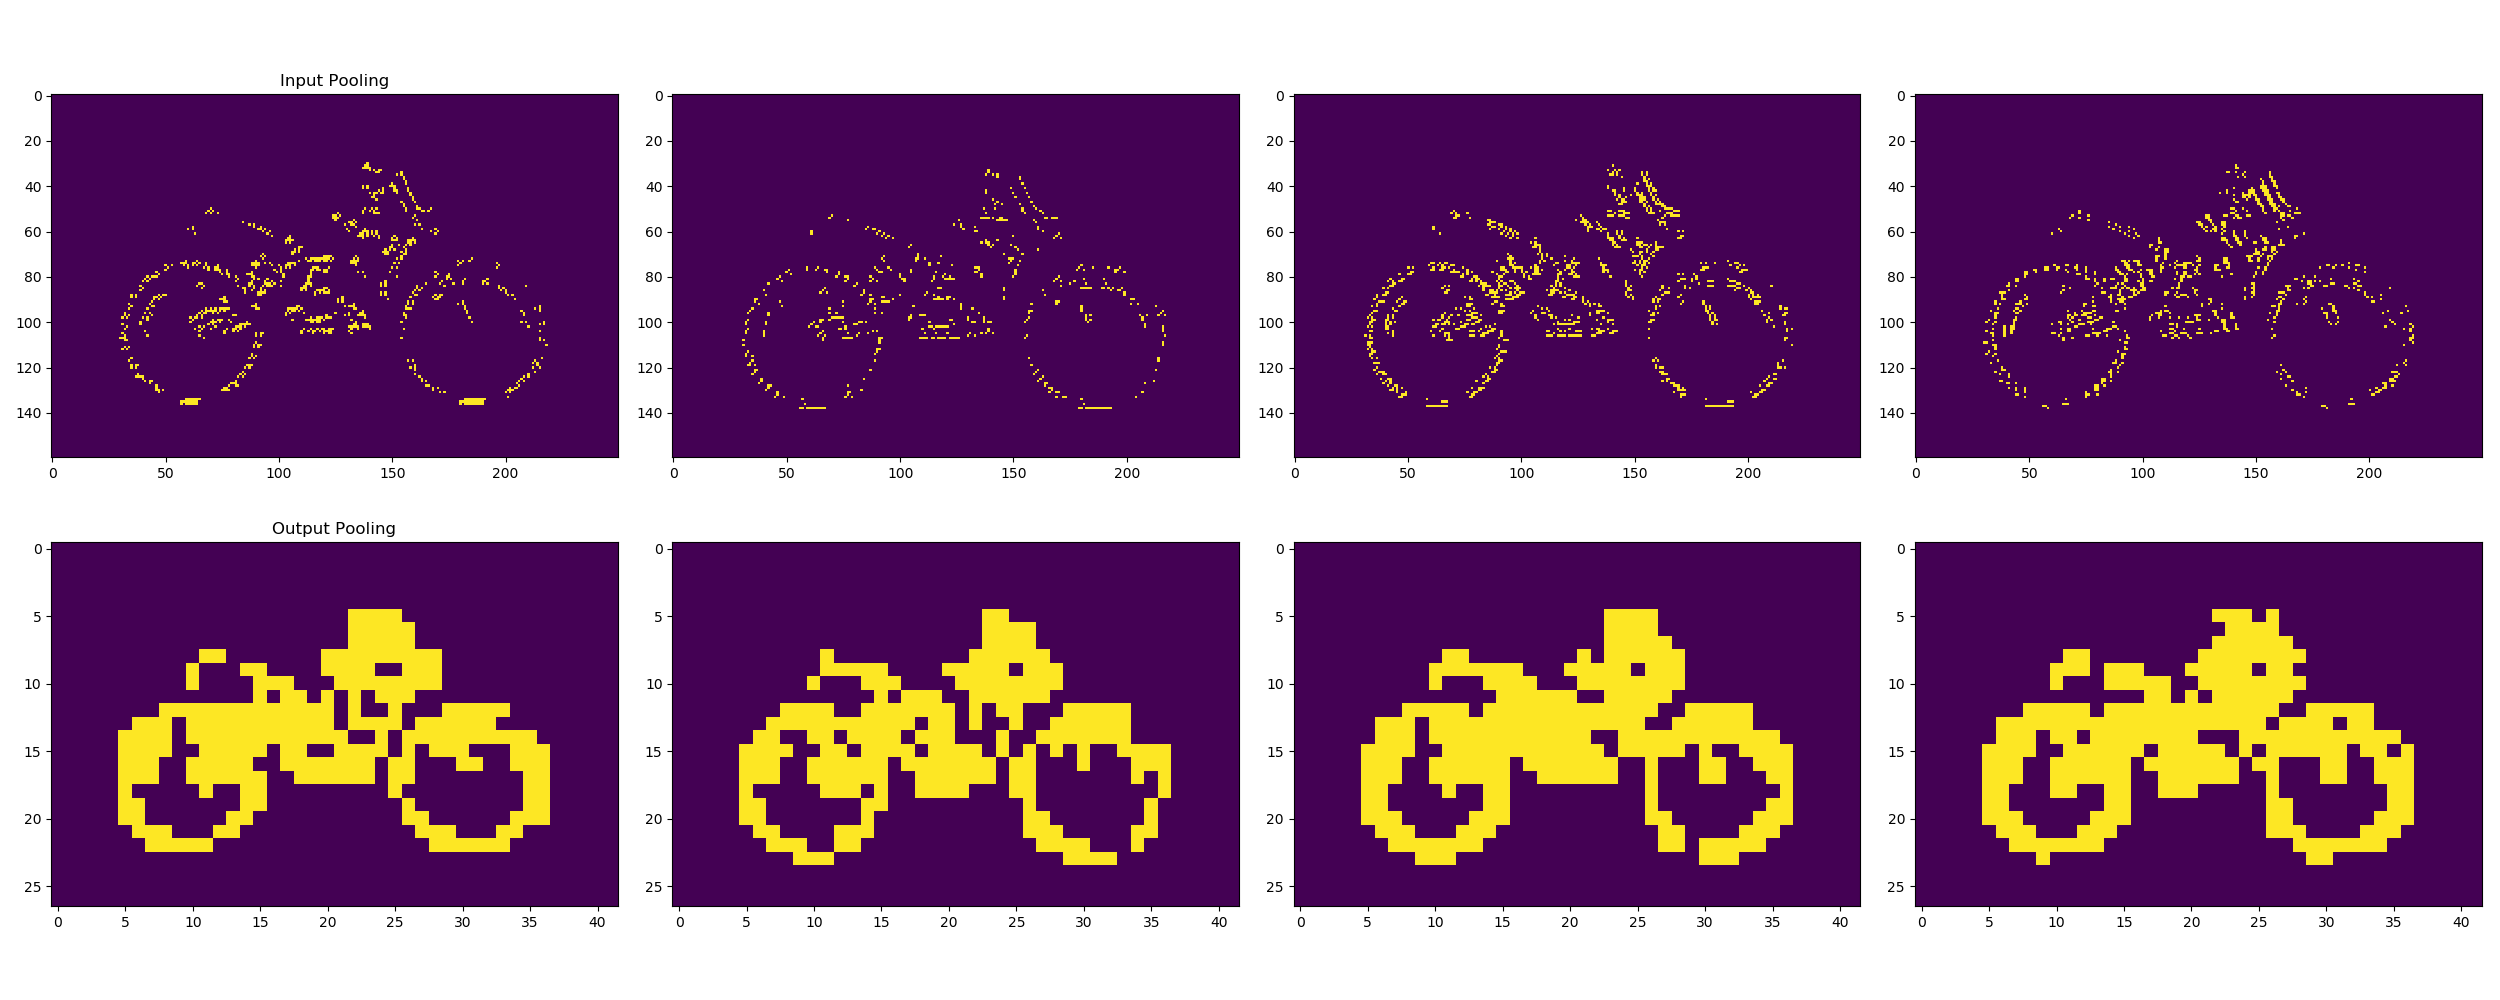
\includegraphics[width=\textwidth]{images/pool_slice1}
	\caption{Input (top) and output (bottom) of the first pooling layer.}
	\label{fig:pool}
\end{figure}\\
As regards the weights, these are randomly initialised and updated after the STDP process. In figure \ref{fig:weights} it is possible to see how the weights change after one and three images are processed. Darker and lighter cells represent lower and higher values (normalised between 0 and 1), respectively.
\begin{figure}[!h]
	\centering
	\begin{minipage}[b]{\textwidth}
		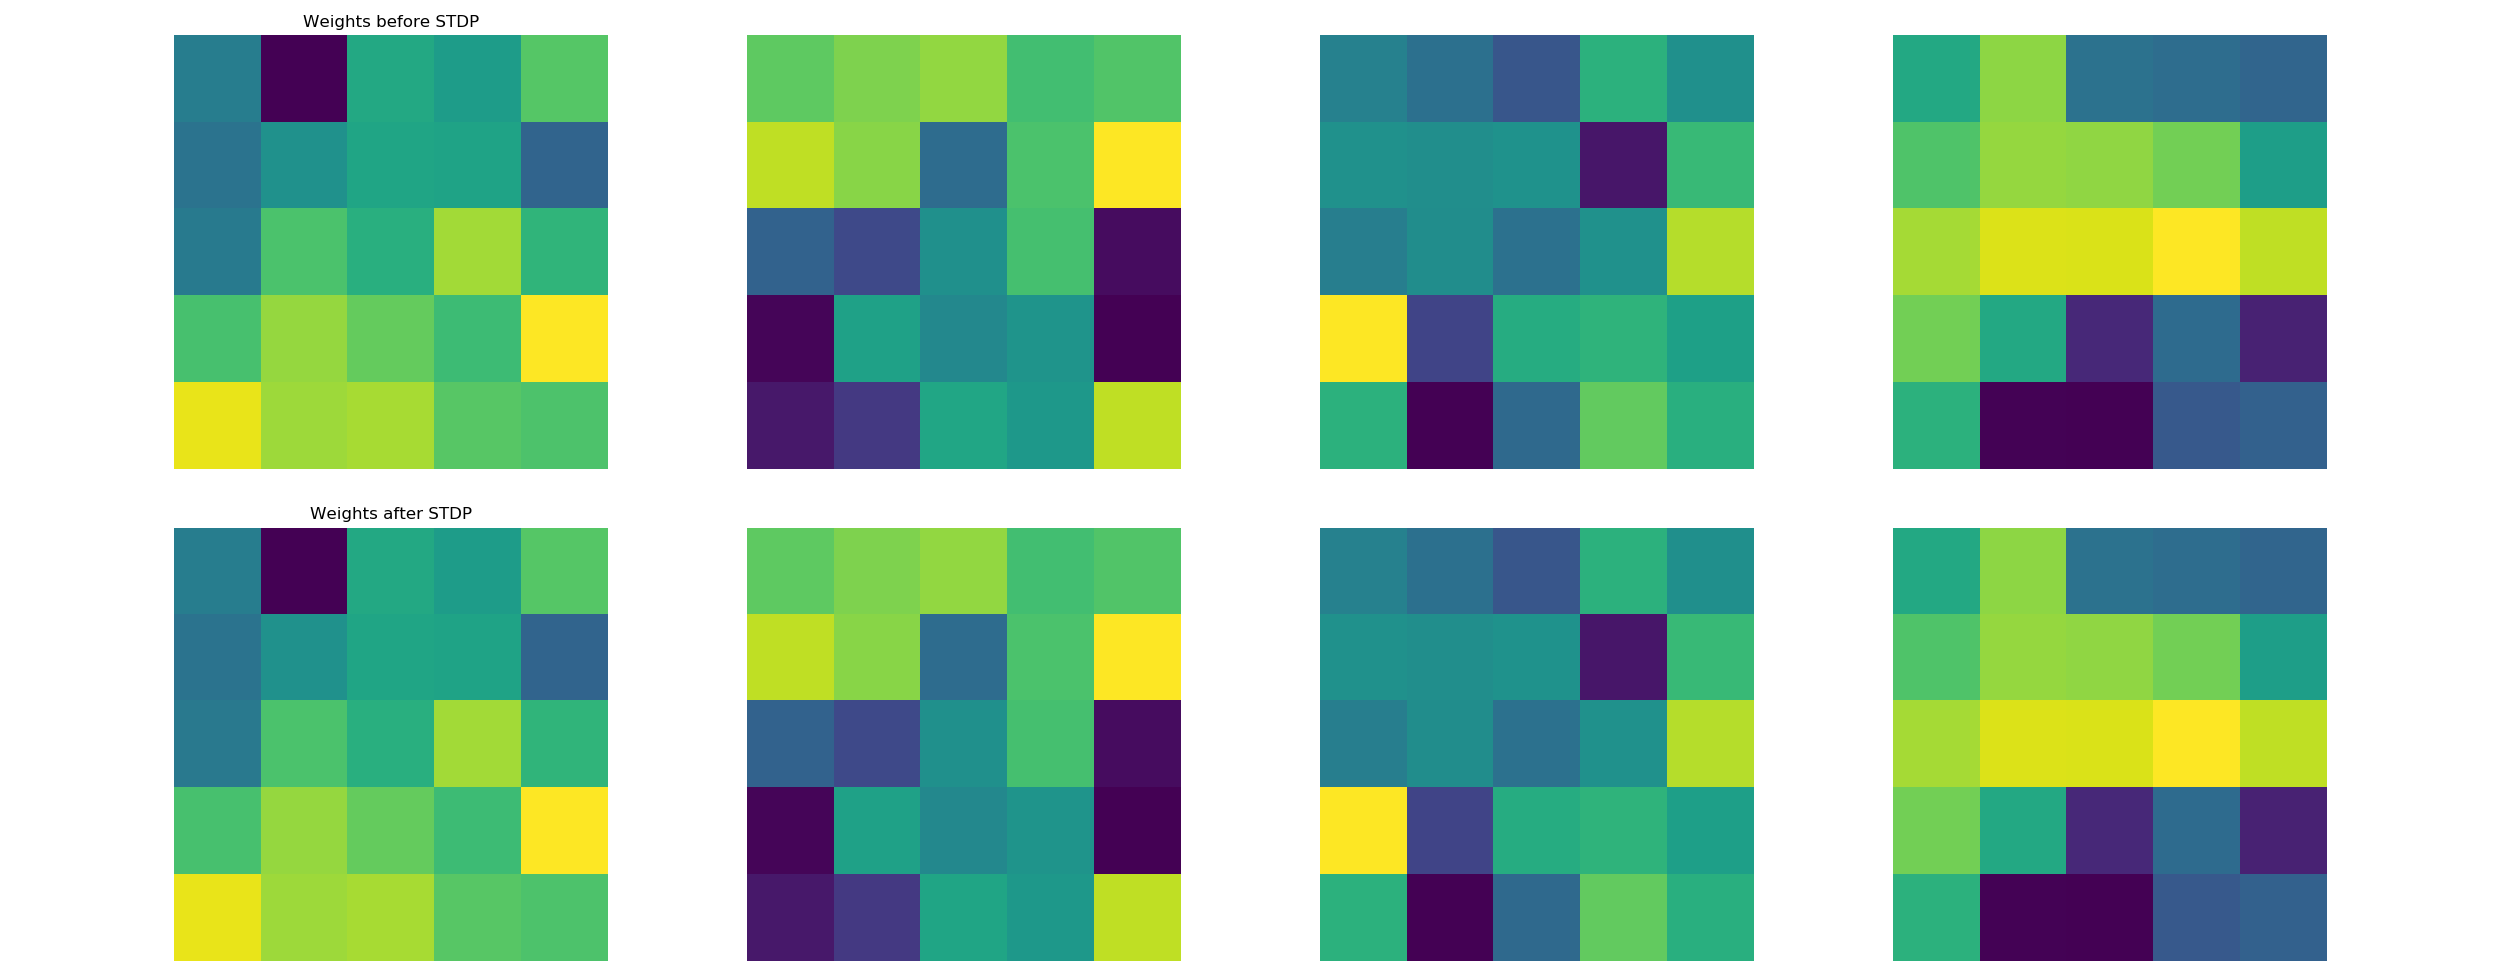
\includegraphics[width=\textwidth]{images/Figure_15}
	\end{minipage}
	\\
	$\:$ \begin{minipage}[b]{\textwidth}
		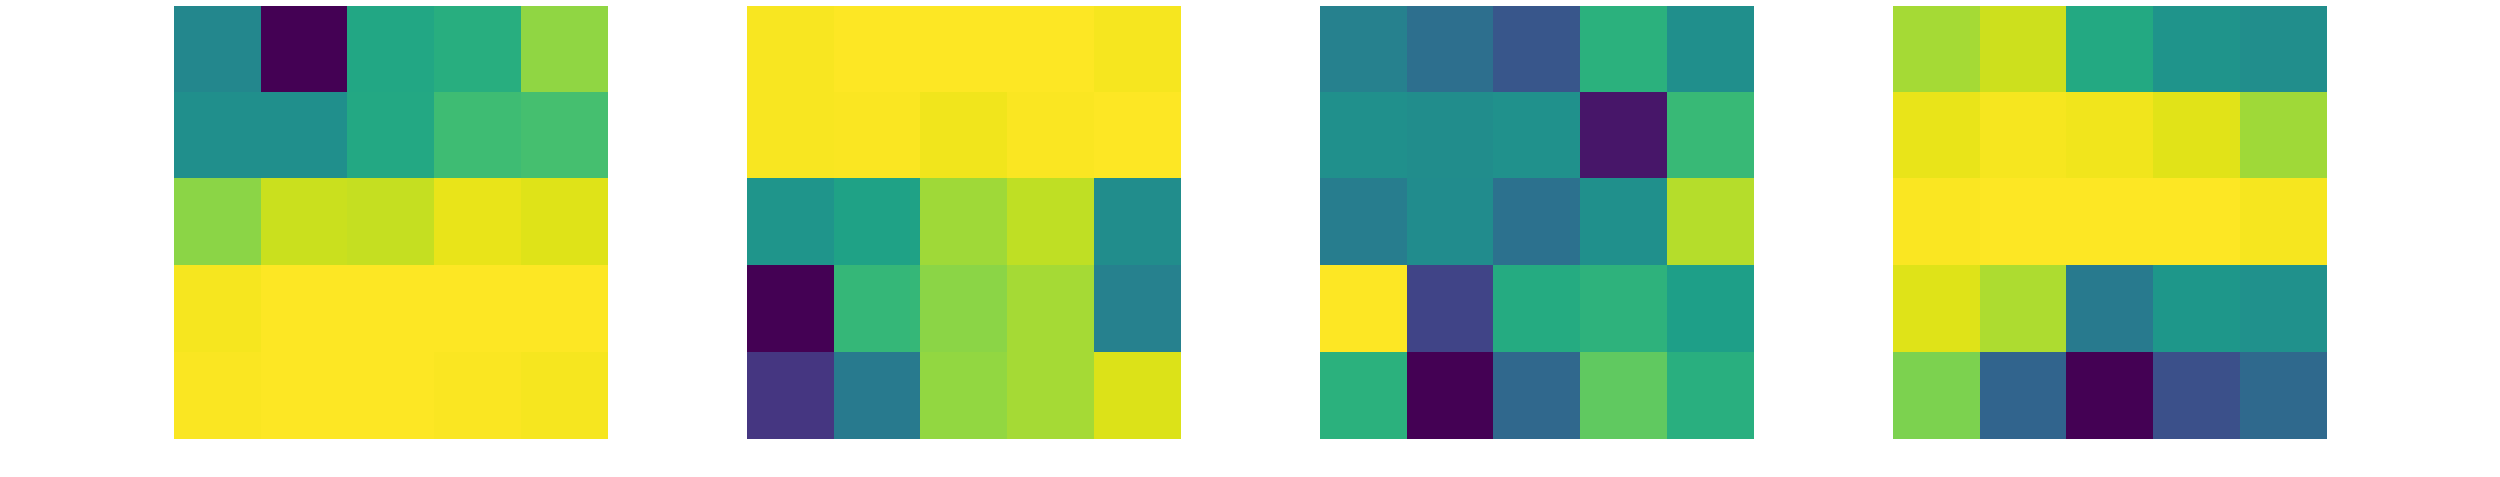
\includegraphics[width=\textwidth]{images/3Figure_15}
	\end{minipage}
	\hfill
	\caption{Top: weights randomly initialised. Middle: weights updated after one image processed. Bottom: weights updated after three image processed}
	\label{fig:weights}
\end{figure}\\
\newpage
Other two convolutional and pooling layers are used before the final classification. To have just an idea of how the data are processed through the network, also the output of the second convolutional layer is shown in figure \ref{fig:conv2}. It is not possible any more to recognize the image after the second convolution.\\
\begin{figure}[!h]
	\centering
	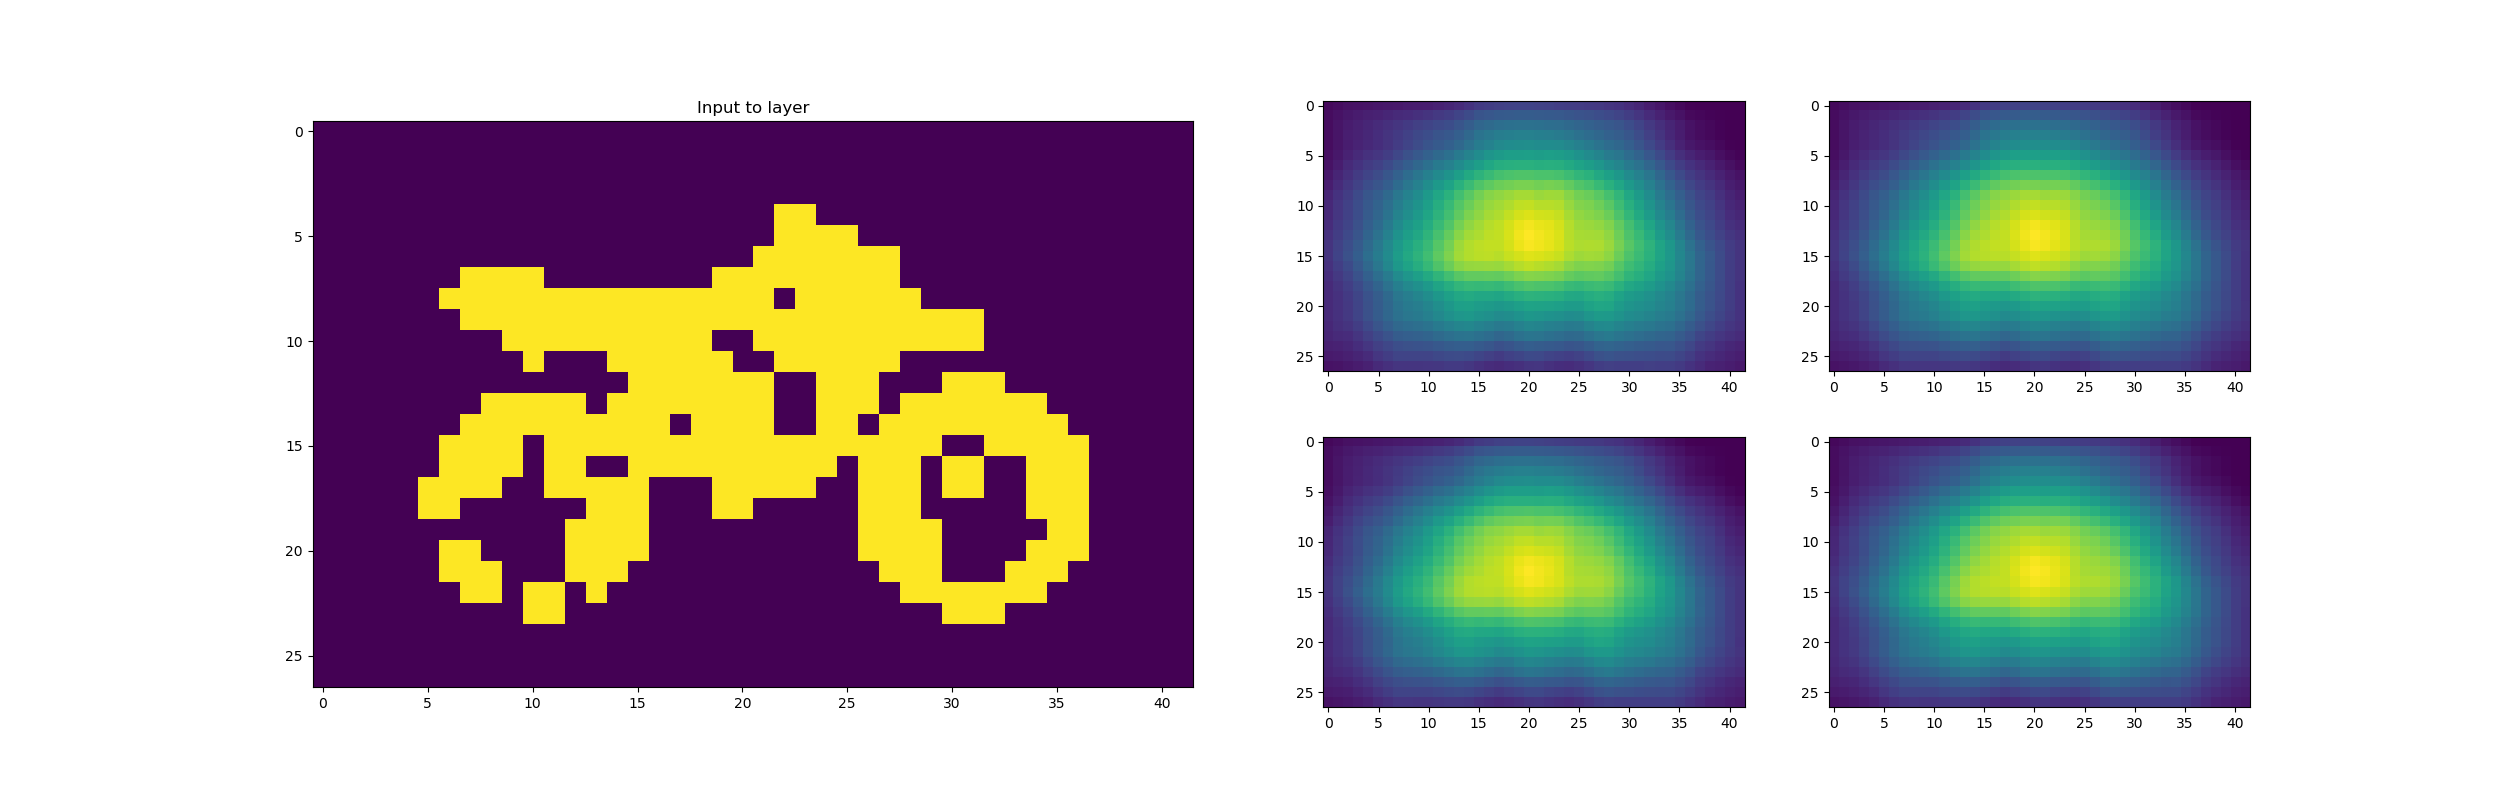
\includegraphics[width=\textwidth]{images/Figure_10}
	\caption{Left: Output of the first pooling layer. Rigth (four images): Output of the second convolutional layer}
	\label{fig:conv2}
\end{figure}
\section{Conclusions}

The new method developed allows to handle the complexity of a bio-inspired neural network by using new spiking neuron models. With respect to classic approaches, it is possible to acquire spatio-temporal information in a better way and obtain good results with few input data.\\
The network has been evaluated several times with different parameters. By taking inspiration from some existing functions the 88\% of accuracy has been obtained. Instead, with all functions implemented from scratch, the score obtained oscillates between 62\% and 75\% (the value strongly depends on the parameters and the classifier used). However, room for improvements is still possible.\\
A possible way is by modifying the STDP, in order to apply penalty on more neurons that are not involved in the spiking process. Another improvement can be made by extending the encoding time of the DoG filter, so as to have a better differentiation between useful and useless information, with the side-effect of a higher computational effort needed.\\
According to the authors of the original paper, there is no other spiking deep network at the moment which can recognize large-scale natural objects. So, even if it is not easy to find better ways of improvements, there is good potential for future breakthroughs. 

\clearpage

\begin{thebibliography}{5}

\bibitem{STPD} 
S. R. Kheradpisheh, M. Ganjtabesh, S. J. Thorpe, and
T. Masquelier, "Stdp-based spiking deep convolutional neural
networks for object recognition," Neural Networks, vol. 99,
pp. 56–67, 2017.

\bibitem{Next-gen}
Spiking Neural Networks, the Next Generation of Machine Learning, https://towardsdatascience.com/spiking-neural-networks-the-next-generation-of-machine-learning-84e167f4eb2b

\bibitem{GitHub}
Spiking-Neural-Network, https://github.com/Shikhargupta/Spiking-Neural-Network
\end{thebibliography}

\end{document}